\clearpage
\newpage

\subsubsection{Estensione F: Riattivazione Notifiche dalle Notifiche Disattivate}

Questa estensione consente all’utente di riattivare una categoria di notifiche direttamente da una notifica precedentemente ricevuta e appartenente a una categoria disattivata. L’obiettivo è fornire un meccanismo immediato per ripristinare le notifiche quando l’utente si rende conto della loro utilità.

\vspace{0.5cm}
\subsubsection{Indicazione dello Stato e Call-to-Action}
Quando una notifica proviene da una categoria disattivata, il sistema mostra un messaggio di avviso evidenziato che informa l’utente che non riceverà più aggiornamenti simili. Il pulsante associato cambia stato e diventa un invito all’azione con il testo “Riattiva notifiche”. Questo sfrutta il \textbf{principio della reversibilità} \cite{shneiderman2004}, permettendo all’utente di annullare la decisione precedente senza difficoltà.

\vspace{0.5cm}
\subsubsection{Feedback Visivo e Conferma della Riattivazione}
Alla pressione del pulsante, il testo cambia colore in verde e il messaggio informativo si aggiorna, confermando che le notifiche per quella categoria sono state riattivate. Il sistema può fornire un’ulteriore conferma con un breve messaggio di notifica o una vibrazione del dispositivo per enfatizzare l’azione completata.

\vspace{0.5cm}
\subsubsection{Coerenza con il Modello di Gestione Notifiche}
Questa estensione rafforza la coerenza dell’interfaccia di gestione delle notifiche, mantenendo le scelte dell’utente sempre modificabili e promuovendo un’interazione trasparente e prevedibile. L’utente può così gestire le notifiche senza dover accedere necessariamente alla schermata delle impostazioni, riducendo il carico cognitivo e migliorando l’usabilità complessiva del sistema.\begin{figure}[ht]
    \centering
    \begin{tikzpicture}[node distance=1.5cm and 1cm, auto]
        % Nodo per immagine 1 con didascalia sotto
        \node (img1) {
            \begin{tabular}{c}
                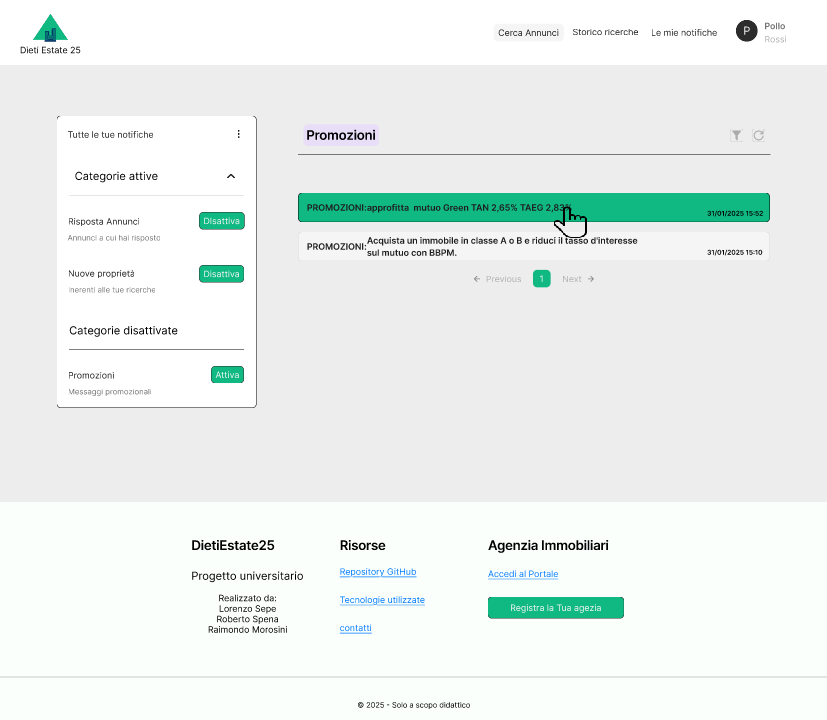
\includegraphics[width=0.4\textwidth]{Immagini/Mockup/notifiche/estensione F/clickNotifica.png} \\
                Cockburn: Extension F.2
            \end{tabular}
        };
        
        % Nodo per immagine 2 con didascalia sotto, posizionato a destra di img1
        \node (img2) [below=of img1] {
            \begin{tabular}{c}
                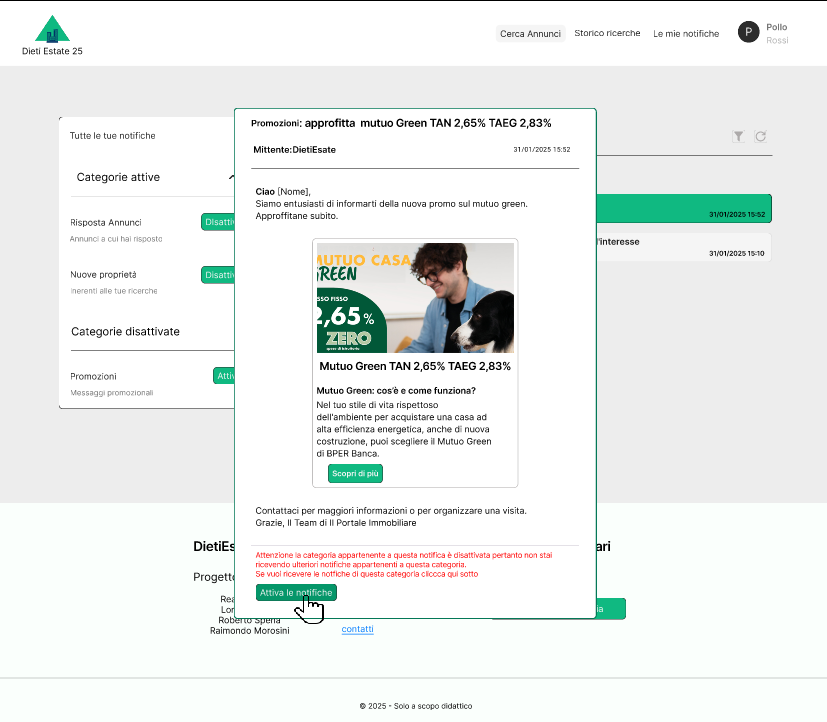
\includegraphics[width=0.4\textwidth]{Immagini/Mockup/notifiche/estensione F/clickAttiva.png} \\
                Cockburn: Extension F.3
            \end{tabular}
        };
        
        % Nodo per immagine 3 con didascalia sotto, posizionato sotto img2
        \node (img3) [below=of img2] {
            \begin{tabular}{c}
                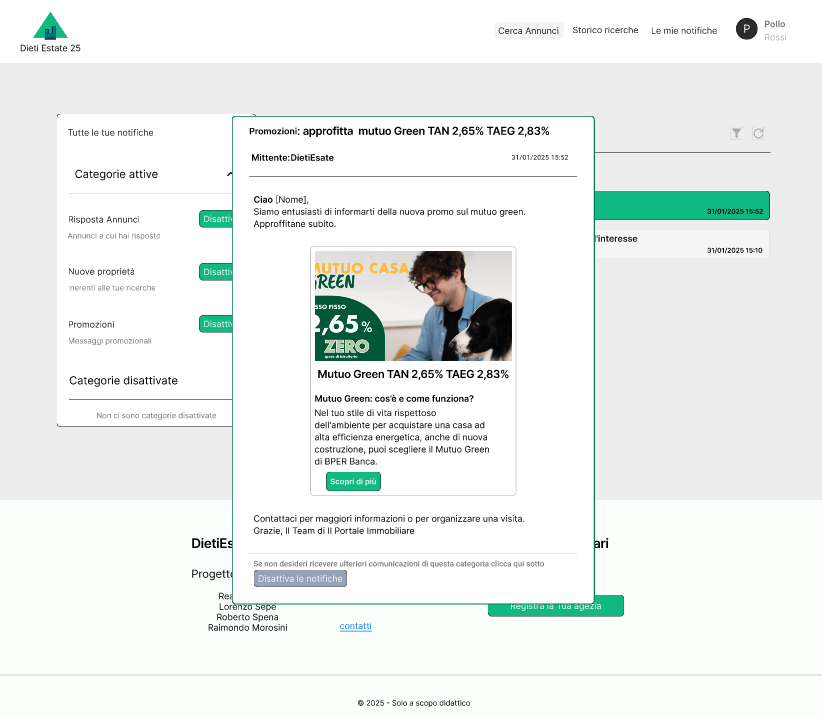
\includegraphics[width=0.4\textwidth]{Immagini/Mockup/notifiche/estensione F/attivato.png} \\
                Cockburn: Extension F.4/F.5
            \end{tabular}
        };
        
        % Disegna le frecce
        \draw[->, thick] (img1) -- (img2);
        \draw[->, thick] (img2) -- (img3);
      
    \end{tikzpicture}
    \caption{Mockup: estensione F della tabella di Cockburn del caso d'uso disattiva/attiva categoria notifica}
    \label{fig:mockup_estensione_F_disattiva_notifiche}
\end{figure}

\newpage

